\documentclass[a4j, uplatex, fleqn, dvipdfmx]{jsarticle} % fleqnで数式を左に寄せる,中央揃えにしたい数式は「ceqn環境(nccmath)」に入れればよい
% \documentclass[a4j, uplatex, twocolumn, fleqn, dvipdfmx]{jsarticle} % fleqnで数式を左に寄せる,中央揃えにしたい数式は「ceqn環境(nccmath)」に入れればよい
\usepackage[dvipdfmx]{graphicx, color}
\usepackage{bm} % 太字
\usepackage{amsmath,amssymb} % 行列など
\usepackage{here} % 画像を入れたい場所に入れられる
\usepackage{fancybox,ascmac} % itembox用
\usepackage{hhline} % 表組の2重線を思い通りにできる
\usepackage{siunitx} % SI単位系
\usepackage{subcaption}
\usepackage{enumitem} % enumerate の item を参照したり見た目を整えたりできる

\usepackage[dvipdfmx, hidelinks]{hyperref} % hidelinksでリンクに色や枠が付かないようにする
\usepackage{pxjahyper}
\hypersetup{% hyperrefオプションリスト
  setpagesize=false, % 不具合回避
  bookmarksnumbered=true, % ブックマークに番号を付ける
  bookmarksopen=true, % pdfのブックマークのツリーをデフォルトで開く(コンパイル環境によっては機能しないらしい)
  colorlinks=true,
  linkcolor=black,
  citecolor=blue,
  urlcolor=cyan
}

% きれいな丸囲み数字
\usepackage{pifont}

%余白は上下30mm、左右20mm
\setlength{\textheight}{\paperheight}
\setlength{\topmargin}{4.6truemm}
\addtolength{\topmargin}{-\headheight}
\addtolength{\topmargin}{-\headsep}
\addtolength{\textheight}{-60truemm}

\setlength{\textwidth}{\paperwidth}
\setlength{\oddsidemargin}{-5.4truemm}
\setlength{\evensidemargin}{-5.4truemm}
\addtolength{\textwidth}{-40truemm}

\title{\vspace{-1.5cm}数理脳科学\\ボルツマンマシン}
% \title{汎用的学習ゲームプラットフォームの作成}
\author{宮崎大学 工学研究科 工学専攻 情報\\T2103329 東郷 拓弥}
% \date{} % タイトルの日付を非表示にする
\begin{document}
\maketitle
\section{問題設定}
素子数 $n = 3$ のボルツマン機械を考えよう.この機械の $j$ 番目の素子から $i$ 番目の素子への結合を
 $w_{ij}$.状態を $x = (x1, x2,x3)$ , $x_i \in {0, 1}$ と書く. 
ここで,結合は対称であり( $w_{ij} = w_{ji}$ ),自己結合はないとする( $w_{ii} = 0$ ).
各素子は非同期的に以下の確率にしたがい自分の状態を変えていく.
\begin{eqnarray}
  \label{eq:excitement_dynamics}
  \operatorname{Pr}\{x_i = 1\} & = & \frac{1}{1 + \exp \{-u_i / T\}}, \qquad \operatorname{Pr}\{x_i = 0\} = 1 - \operatorname{Pr}\{x_i = 1\} \\
  u_i & = & \sum_{j=1}^n w_{ij} x_j - h_i = \sum_{j=0}^n w_{ij} x_j
\end{eqnarray}
ここで,常に興奮している素子 $x_0 = 1$ を仮想的に考え,しきい値を $h_i = −w_{i0}$ と表現し記述を簡潔にした.
パラメータ $T$ の値は,以下では特別な指示がなければ $T = 1$ とする.
時間 $t$ における回路の状態を $\bm{x}(t)$ と書こう. 回路の状態は,
$ \bm{x}(0) \rightarrow \bm{x}(1) \rightarrow \bm{x}(2) \rightarrow \bm{x}(3) \rightarrow \cdots $
と,マルコフ連鎖として状態遷移を続けていく.これは次の定常分布
\begin{equation}
  \label{eq:stationary_distribution}
  p(\bm{x} ; \bm{w}) = c \exp \{-E(\bm{x} ; \bm{w}) / T\}
\end{equation}
をもつことが知られている.ここで
\begin{align}
  E(\bm{x} ; \bm{w}) &=-\sum_{i<j} w_{i j} x_{i} x_{j} \\
  &=-\left(w_{01} x_{1}+w_{02} x_{2}+w_{03} x_{3}+w_{12} x_{1} x_{2}+w_{13} x_{1} x_{3}+w_{23} x_{2} x_{3}\right)
\end{align}
であり,$c$ は $\sum_{\bm{x}} p(\bm{x}; \bm{w}) = 1$ とするための正規化定数
\begin{equation}
  c = c(\bm{w}) = \frac{1}{\sum_{\tilde{\bm{x}}} \exp \{-E(\tilde{\bm{x}} ; \bm{w}) / T\}}
\end{equation}
$\bm{w}$ はパラメータ $\bm{w} = (w_{01}, \cdots , w_{23})$ である.回路の性質は $\bm{w}$ で決まる.
以下,素子数 $n = 3$の場合を考える.
コンピュータプログラムは,素子数が $n = 4, 5, \cdots$ となる場合にも簡単に対応できるよう書ければよいが,無理はしなくてよい
($n = 16$ とか $n = 32$ の場合のシミュレーションができればよいが,2 進数と 10 進数を変換する関数を書く必要がある).



\section{問1}
\subsection{問題文}
初期状態として回路に適当な興奮状態を設定した場合,\eqref{eq:excitement_dynamics}式にしたがい状態が変化していく.
素子数 $n = 3$ の場合, $2^3 = 8$ 個の状態 ($\bm{x}_0 \sim \bm{x}_7$,表 1 参照)をとりうる.
それぞれの状態が\eqref{eq:stationary_distribution}式の確率で出現するか,以下の (a),(b),(c) 3 通りについて計算機実験で確認し,表 \ref{table:q1_a_sample},表 \ref{table:q1_b_sample},表 \ref{table:q1_c_sample} を完成させよ.
\begin{enumerate}[label=(\alph{enumi}), ref=(\alph{enumi})]
  % \renewcommand{\labelenumi}{(\alph{enumi}) }
  \item \label{item:q1_a}
    どの素子も互いに結合していないとする($w_{ij} = 0, i, j = 0, \cdots, 3$).
    この場合,式\eqref{eq:stationary_distribution}の定常分布を計算すると, どの状態も確率 $\frac{1}{8}$ で出現することがわかる. 
    実際に計算機シミュレーションをおこない,出現頻度を確かめよ(表\ref{table:q1_a_sample}).
  \item \label{item:q1_b}
    結合係数 $\bm{w} = {w_{ij}}$ の値をランダムな値に設定し(たとえば $[-5:5]$ の一様分布にしたがう乱数.ただし $w_{ii} = 0, w_{ij} = w_{ji}$ とする),
    式\eqref{eq:stationary_distribution}の定常分布を計算し,各状態の出現確率を求めよ.
    また,実際に計算機シミュレーションをおこない,出現頻度を確かめよ(表\ref{table:q1_b_sample}).
  \item \label{item:q1_c} 
    状態 $\bm{x}^3$ と状態 $\bm{x}^6$ だけが出現するような回路を作ることはできるだろうか.
    相関型連想記憶で記憶パターンを埋め込んだように$w_{i j}=\sum_{\bm{x}^{3}, \bm{x}^{6}}\left(2 x_{i}-1\right)\left(2 x_{j}-1\right)$としてみよう.
    学習前の結合係数が $w_{ij} = 0, i, j = 0, \cdots, n$ である場合,学習後の各係数の具体的な値を求めよ($w_{ij} = w_{ji}$ であるので,以下では $i < j$ のみ記述を求めている).
    この {$w_{ij}$} と式\eqref{eq:stationary_distribution}を用い,定常分布における各状態の $p(\bm{x})$(理論値.ボルツマン分布)を計算せよ.
    また,コンピュータシミュレーションをおこない,各状態が実際に出現した頻度を計算し,それを理論値と比較せよ
    (表 \ref{table:q1_c_sample}.繰り返し回数 $l$ を 1 万,100 万などと変えて,少なくとも 2 通りは試すこと).
\end{enumerate}
% 表1
\begin{table}[H]
  \caption{機械の定常状態(結合なし)}
  \label{table:q1_a_sample}
  \centering
  \begin{tabular}{|c|c|c|c|}
    \hline
     & 状態$\bm{x}$ & 出現回数 & 出現頻度 \\
    \hline
    $\bm{x}^{0}$ & $(0,0,0)$ & & \\
    $\bm{x}^{1}$ & $(0,0,1)$ & & \\
    $\bm{x}^{2}$ & $(0,1,0)$ & & \\
    $\bm{x}^{3}$ & $(0,1,1)$ & & \\
    $\bm{x}^{4}$ & $(1,0,0)$ & & \\
    $\bm{x}^{5}$ & $(1,0,1)$ & & \\
    $\bm{x}^{6}$ & $(1,1,0)$ & & \\
    $\bm{x}^{7}$ & $(1,1,1)$ & & \\
    \hline
  \end{tabular}
\end{table}

% 表2
\begin{table}[H]
  \caption{機械の定常状態(ランダム結合の場合)}
  \label{table:q1_b_sample}
  \centering
  \begin{tabular}{|c|c|c|c|c|}
    \hline
     & 状態 $\bm{x}$ & 理論値: $p(\bm{x} ; \bm{w})$ & 実験値: $p(\bm{x} ; \bm{w})$ & 実験値: $p(\bm{x} ; \bm{w})$ \\
     & & & $l=1,000$ & $l=1,000,000$ \\
    \hline
    $\bm{x}^{0}$ & $(0,0,0)$ & & & \\
    $\bm{x}^{1}$ & $(0,0,1)$ & & & \\
    $\bm{x}^{2}$ & $(0,1,0)$ & & & \\
    $\bm{x}^{3}$ & $(0,1,1)$ & & & \\
    $\bm{x}^{4}$ & $(1,0,0)$ & & & \\
    $\bm{x}^{5}$ & $(1,0,1)$ & & & \\
    $\bm{x}^{6}$ & $(1,1,0)$ & & & \\
    $\bm{x}^{7}$ & $(1,1,1)$ & & & \\
    \hline
  \end{tabular}
\end{table}

% 表3
\begin{table}[H]
  \caption{機械の定常状態(連想記憶もどき)}
  \label{table:q1_c_sample}
  \centering
  \begin{tabular}{|r|c|c|c|c|}
    \hline
     & 状態 $\bm{x}$ & 理論値: $p(\bm{x} ; \bm{w})$ & 実験値: $p(\bm{x} ; \bm{w})$ & 実験値: $p(\bm{x} ; \bm{w})$ \\
     & & & $l=1,000$ & $l=1,000,000$ \\
    \hline
    $            \bm{x}^{0}$ & $(0,0,0)$ & & & \\
    $            \bm{x}^{1}$ & $(0,0,1)$ & & & \\
    $            \bm{x}^{2}$ & $(0,1,0)$ & & & \\
    $\rightarrow \bm{x}^{3}$ & $(0,1,1)$ & & & \\
    $            \bm{x}^{4}$ & $(1,0,0)$ & & & \\
    $            \bm{x}^{5}$ & $(1,0,1)$ & & & \\
    $\rightarrow \bm{x}^{6}$ & $(1,1,0)$ & & & \\
    $            \bm{x}^{7}$ & $(1,1,1)$ & & & \\
    \hline
  \end{tabular}
\end{table}

\subsection{回答}
\subsubsection{\ref{item:q1_a}}
結合係数を全て0とし実際に100万回シミュレーションを行ったところ、表\ref{table:q1_a}のようになった。

% 表1_埋めた
\begin{table}[H]
  \caption{機械の定常状態(結合なし)}
  \label{table:q1_a}
  \centering
  \begin{tabular}{|c|c|c|c|}
    \hline
     & 状態$\bm{x}$ & 出現回数 & 出現頻度 \\
    \hline
    $\bm{x}^{0}$ & $(0,0,0)$ & 125221 & 0.125221 \\
    $\bm{x}^{1}$ & $(0,0,1)$ & 125772 & 0.125772 \\
    $\bm{x}^{2}$ & $(0,1,0)$ & 124731 & 0.124731 \\
    $\bm{x}^{3}$ & $(0,1,1)$ & 125890 & 0.125890 \\
    $\bm{x}^{4}$ & $(1,0,0)$ & 124479 & 0.124479 \\
    $\bm{x}^{5}$ & $(1,0,1)$ & 124638 & 0.124638 \\
    $\bm{x}^{6}$ & $(1,1,0)$ & 124036 & 0.124036 \\
    $\bm{x}^{7}$ & $(1,1,1)$ & 125233 & 0.125233 \\
    \hline
  \end{tabular}
\end{table}

どのパターンも誤差$\pm 0.001$以内で$\frac{1}{8}$の確率で出現し、理論通りの結果となった。


\subsubsection{\ref{item:q1_b}}
結合係数を$[-5:5]$ の一様分布にしたがう乱数により初期化し、表\ref{table:q1_b_sample}を埋めたところ、表\ref{table:q1_b}のようになった。

% 表2_埋めた
\begin{table}[htb]
  \caption{機械の定常状態(ランダム結合の場合)}
  \label{table:q1_b}
  \centering
  \begin{tabular}{|c|c|r|r|r|r|}
    \hline
     & 状態 $\bm{x}$ & 理論値: $p(\bm{x} ; \bm{w})$ & 実験値: $p(\bm{x} ; \bm{w})$ & 実験値: $p(\bm{x} ; \bm{w})$ & 実験値: $p(\bm{x} ; \bm{w})$ \\
     & & & $l=1,000$ & $l=1,000,000$ & $l=10,000,000$ \\
    \hline
    $\bm{x}^{0}$ & $(0,0,0)$ & 8.85748763e-01 & 0.888 & 8.86341e-01 & 8.860349e-01 \\
    $\bm{x}^{1}$ & $(0,0,1)$ & 7.04071483e-03 & 0.006 & 7.39600e-03 & 7.035400e-03 \\
    $\bm{x}^{2}$ & $(0,1,0)$ & 8.99050110e-03 & 0.009 & 9.14200e-03 & 8.939600e-03 \\
    $\bm{x}^{3}$ & $(0,1,1)$ & 4.94892468e-07 & 0.    & 0.00000e+00 & 7.000000e-07 \\
    $\bm{x}^{4}$ & $(1,0,0)$ & 8.86149417e-02 & 0.08  & 8.74730e-02 & 8.836140e-02 \\
    $\bm{x}^{5}$ & $(1,0,1)$ & 6.99043265e-03 & 0.006 & 6.96700e-03 & 7.025500e-03 \\
    $\bm{x}^{6}$ & $(1,1,0)$ & 2.61272433e-03 & 0.011 & 2.68000e-03 & 2.600700e-03 \\
    $\bm{x}^{7}$ & $(1,1,1)$ & 1.42728741e-06 & 0.    & 1.00000e-06 & 1.800000e-06 \\
    \hline
  \end{tabular}
\end{table}

確率が著しく小さい値があったが、定常分布を計算した値とシミュレーションの結果は概ね等しくなった。

\subsubsection{\ref{item:q1_c}}
$\bm{x}^{3}=(0, 1, 1), \bm{x}^{6} = (1, 1, 0)$を考慮し、
$w_{i j}=\sum_{\bm{x}^{3}, \bm{x}^{6}}\left(2 x_{i}-1\right)\left(2 x_{j}-1\right)$を計算した結果、次のようになった。

\begin{alignat*}{4}
  w_{01} &= (2-1)(0-1) + (2-1)(2-1) & &= -1 +1 & &=  0 \\
  w_{02} &= (2-1)(2-1) + (2-1)(2-1) & &=  1 +1 & &=  2 \\
  w_{03} &= (2-1)(2-1) + (2-1)(0-1) & &=  1 -1 & &=  0 \\
  w_{12} &= (0-1)(2-1) + (2-1)(2-1) & &= -1 +1 & &=  0 \\
  w_{13} &= (0-1)(2-1) + (2-1)(0-1) & &= -1 -1 & &= -2 \\
  w_{23} &= (2-1)(2-1) + (2-1)(0-1) & &=  1 -1 & &=  0
\end{alignat*}

これを初期値として回路を作成し、シミュレーションを行った。

% 表3_埋めた
\begin{table}[htb]
  \caption{機械の定常状態(連想記憶もどき)}
  \label{table:q1_c}
  \centering
  \begin{tabular}{|r|c|r|r|r|}
    \hline
     & 状態 $\bm{x}$ & 理論値: $p(\bm{x} ; \bm{w})$ & 実験値: $p(\bm{x} ; \bm{w})$ & 実験値: $p(\bm{x} ; \bm{w})$ \\
     & & & $l=1,000$ & $l=1,000,000$ \\
    \hline
    $            \bm{x}^{0}$ & $(0,0,0)$ & 0.03801919 & 0.033 & 0.038053 \\
    $            \bm{x}^{1}$ & $(0,0,1)$ & 0.03801919 & 0.052 & 0.037384 \\
    $            \bm{x}^{2}$ & $(0,1,0)$ & 0.28092596 & 0.311 & 0.281948 \\
    $\rightarrow \bm{x}^{3}$ & $(0,1,1)$ & 0.28092596 & 0.243 & 0.280352 \\
    $            \bm{x}^{4}$ & $(1,0,0)$ & 0.03801919 & 0.05  & 0.038028 \\
    $            \bm{x}^{5}$ & $(1,0,1)$ & 0.00514534 & 0.006 & 0.005136 \\
    $\rightarrow \bm{x}^{6}$ & $(1,1,0)$ & 0.28092596 & 0.279 & 0.280848 \\
    $            \bm{x}^{7}$ & $(1,1,1)$ & 0.03801919 & 0.026 & 0.038251 \\
    \hline
  \end{tabular}
\end{table}

理論値、実験値共に
状態 $\bm{x}^3$ と状態 $\bm{x}^6$ だけが出現するような回路にはならなかった.

\section{問2}
\subsection{問題文}
各状態 $\bm{x}$ が次の表 \ref{table:q2} に示す頻度で出現するボルツマン機械を,学習により実現しよう.

% 表4
\begin{table}[H]
  \caption{ボルツマン機械の学習.信号 x の出現頻度.}
  \label{table:q2}
  \centering
  \begin{tabular}{|c|c|r|r|}
    \hline
     & 状態$\bm{x}$ & 外界(真の分布): $q(\bm{x})$ & 機械が実現する分布 $p(\bm{x}; \{w_{ij}\})$ \\
    \hline
    $\bm{x}^{0}$ & (0,0,0) & 0.1 & \\
    $\bm{x}^{1}$ & (0,0,1) & 0.1 & \\
    $\bm{x}^{2}$ & (0,1,0) & 0.05 & \\
    $\bm{x}^{3}$ & (0,1,1) & 0.05 & \\
    $\bm{x}^{4}$ & (1,0,0) & 0.1 & \\
    $\bm{x}^{5}$ & (1,0,1) & 0.1 & \\
    $\bm{x}^{6}$ & (1,1,0) & 0.4 & \\
    $\bm{x}^{7}$ & (1,1,1) & 0.1 & \\
    \hline
  \end{tabular}
\end{table}


\begin{enumerate}[label=(\alph{enumi}), ref=(\alph{enumi})]
  \item 
    すべての結合係数を $w_{ij} = 0$ とする(乱数でもよい).
  \item 
    表 \ref{table:q2} に示す確率分布 $q(\bm{x})$ にしたがい $\bm{x}$ を 100 個生成する.
    $x_i$ と $x_j$ が同時に 1 をとる頻度を $f_{ij}$ とせよ.(こんな実験をするのは時間の無駄だと思えば,
    期待値 $\sum_{\alpha} x_{i} x_{j} p\left(\bm{x}^{\alpha}\right)$ を計算すればよい.
    $\Rightarrow f_{01} = 0.7, f_{02} = 0.6, f_{03} = 0.35, f_{12} = 0.5, f_{13} = 0.2, f_{23} = 0.15.$
    ここで,$x_0$ は常に 1 であること($x_0 = 1$),
    $\bm{x}$ として,$\bm{x} = (x_1, x_2, x_3)$ と,$x_0$ をのぞいて表記していることに注意.
    ただし信号の次元 $n$ が大きくなると, $2^n$ とおりの状態数を考慮する必要があり,こういう計算はできない.
    その場合は,実際に信号を生成して統計量を計算するしかない).
  \item \label{item:q2_c}
    回路の初期状態を $\bm{x}(0) = (0, 0, 0)$ に設定する.
  \item \label{item:q2_d} 
    ランダムに一つの素子を選び,その素子の状態を更新する.
    これを 100 回繰り返し,素子 $x_i$ と $x_j$ が同時に 1 になった頻度を $g_{ij}$ とする
    (頻度 $g_{ij}$ は同時に 1 になった回数を 100 で割ったもの. $0 \leqq g_{ij} \leqq 1$).
  \item
    結合係数の値を更新する(学習):
    \begin{align}
      w_{i j}:=w_{i j}+0.01\left(f_{i j}-g_{i j}\right)
    \end{align}
  \item 
    Kullback-Leibler のダイバージェンス
    \begin{align}
      D=\sum_{\bm{x}} q(\bm{x}) \log \frac{q(\bm{x})}{p(\bm{x})}
    \end{align}
    を計算する.ここで $p(\bm{x})$ は,実際に回路を自由に走らせて計算してもよいが,
    素子数 $n$ が小さい場合は,回路のパラメータ \{$w_{ij}$\} から計算できる理論値(式\eqref{eq:stationary_distribution})を用いればよい.
  \item 
    \ref{item:q2_d} にもどり繰り返す(繰り返し回数は任意.例えば 10000 回).
  \item \label{item:q2_h}
    横軸に学習回数 $t$, 縦軸に Kullback-Leibler のダイバージェンスをプロットした図を描き(曲線が描ける),
    学習が進むにしたがい $p(\bm{x})$ が $q(\bm{x})$ に近づいていく($D = 0$ に近づく)様子を確認せよ.
  \item \label{item:q2_i}
    獲得した $w_{ij}$ の値を列挙せよ.
  \item \label{item:q2_j}
    しきい値がない $n = 3$ の回路を考えよう($w_{01} = w_{02} = w_{03} = 0$).
    このとき同様な実験をおこない(もう一度 \ref{item:q2_c} から実験をする),結果を比較し考察せよ(2本の曲線の位置関係を比較せよ).
\end{enumerate}

\subsection{回答}
\subsubsection{\ref{item:q2_h}}
手順に従ってボルツマン機械の学習を行ったところ、図\ref{fig:q2_h_graph}のようになった。
\begin{figure}[htbp]
  \centering
  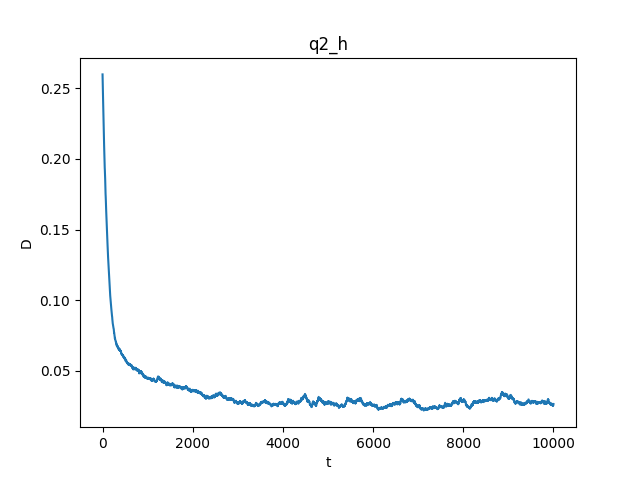
\includegraphics[width=12cm]{images/q2_h_graph.png}
  \caption{Kullback-Leibler}
  \label{fig:q2_h_graph}
\end{figure}


\subsubsection{\ref{item:q2_i}}
獲得した$w_{ij}$の値は、以下のようになった。

$w_{01}=0.1633,\quad w_{02}=-0.6983,\quad w_{03}=0.1486,\quad w_{12}=1.9988,\quad w_{13}=-0.2417,\quad w_{23}=-0.7648$

\subsubsection{\ref{item:q2_j}}
閾値がない回路でボルツマン機械の学習を行ったところ、図\ref{fig:q2_j_graph}のようになった。
\begin{figure}[htbp]
  \centering
  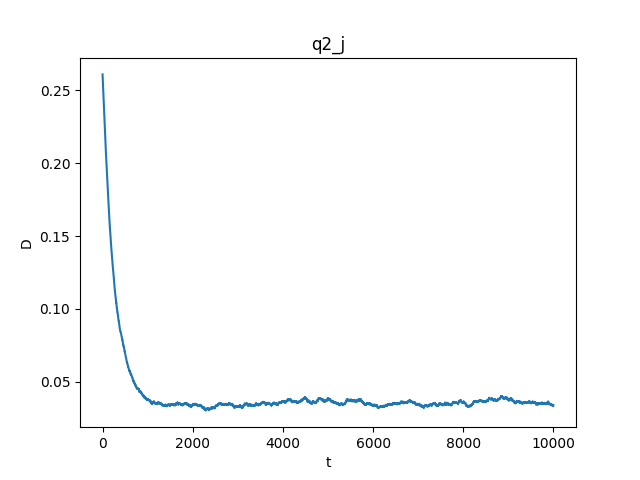
\includegraphics[width=12cm]{images/q2_j_graph.png}
  \caption{Kullback-Leibler}
  \label{fig:q2_j_graph}
\end{figure}

\ref{item:q2_h}と\ref{item:q2_j}で求めた結果を比較できるように、図\ref{fig:q2_j_h_graph}にプロットを行った。
\begin{figure}[htbp]
  \centering
  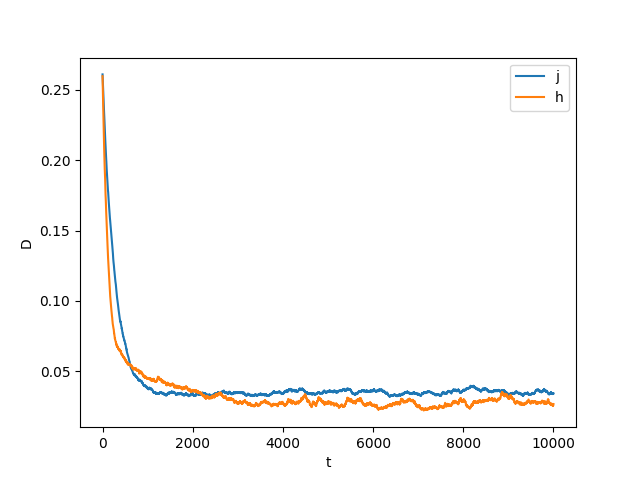
\includegraphics[width=12cm]{images/q2_j_h_graph.png}
  \caption{Kullback-Leibler}
  \label{fig:q2_j_h_graph}
\end{figure}

図\ref{fig:q2_j_h_graph}から、閾値がある回路は閾値がない回路に比べて最終的にKullback-Leibler のダイバージェンスの値が小さくなった。
また、最初のダイバージェンスが大きい間は閾値がない回路よりも結果は良かったが、
ダイバージェンスが0に近づいた時に一時的に学習効率が落ち、ダイバージェンスが閾値がない回路よりも大きくなった。

\section{問3}
\subsection{問題文}
しきい値ありの学習済みの回路において 1 番目の素子の値を $x_1 = 1$ と固定し, $x_2$, $x_3$だけ値の更新を許すとしよう.
このとき,条件付き確率を直接学習したわけではないが,条件付き確率が学習されていることを確かめよ.

% 画像
% \begin{figure}[htbp]
%   \centering
%   \includegraphics[width=12cm]{images/XXX.png}
%   \caption{XXX}
%   \label{fig:XXX}
% \end{figure}

% 画像(横に二枚)
% \begin{figure}[htbp]
%   \centering
%   \begin{tabular}{c}
%     \begin{minipage}{0.45\hsize}
%       \centering
%       \includegraphics[width=7cm]{img/XXX.pdf}
%       \caption{XXX}
%       \label{fig:XXX}
%     \end{minipage}

%     \begin{minipage}{0.45\hsize}
%     \centering
%     \includegraphics[width=7cm]{img/XXX.pdf}
%     \caption{XXX}
%     \label{fig:XXX2}
%     \end{minipage}
% \end{tabular}
% \end{figure}

% 表
% \begin{table}[htb]
%   \caption{XXX}
%   \label{table:XXX}
%   \centering
%   \begin{tabular}{crrr}
%     \hline
%     画像 & 平均画素値(r) & 平均画素値(g) & 平均画素値(b) \\
%     \hline \hline
%     1番目 & 84.557053 & 102.190216 & 107.264511 \\
%     2番目 & 100.516571 & 126.928757 & 138.014618 \\
%     \hline
%   \end{tabular}
% \end{table}

% 画像 マトリックス状 参考:http://www.yamamo10.jp/~yamamoto/comp/latex/make_doc/insert_fig/index.php
% \begin{figure}[htbp]
%   \begin{minipage}[b]{0.32\linewidth}
%     \centering
%     \includegraphics[keepaspectratio, scale=0.3]{images/Q3/xor_sig02.png}
%     \subcaption{$\sigma=0.2$}
%   \end{minipage}
%   \begin{minipage}[b]{0.32\linewidth}
%     \centering
%     \includegraphics[keepaspectratio, scale=0.3]{images/Q3/xor_sig02.png}
%     \subcaption{$\sigma=0.3$}
%   \end{minipage}
%   \begin{minipage}[b]{0.32\linewidth}
%     \centering
%     \includegraphics[keepaspectratio, scale=0.3]{images/Q3/xor_sig05.png}
%     \subcaption{$\sigma=0.5$}
%   \end{minipage}
%   \\
%   \begin{minipage}[b]{0.32\linewidth}
%     \centering
%     \includegraphics[keepaspectratio, scale=0.3]{images/Q3/xor_sig1.png}
%     \subcaption{$\sigma=1$}
%   \end{minipage}
%   \begin{minipage}[b]{0.32\linewidth}
%     \centering
%     \includegraphics[keepaspectratio, scale=0.3]{images/Q3/xor_sig2.png}
%     \subcaption{$\sigma=2$}
%   \end{minipage}
%   \begin{minipage}[b]{0.32\linewidth}
%     \centering
%     \includegraphics[keepaspectratio, scale=0.3]{images/Q3/xor_sig3.png}
%     \subcaption{$\sigma=3$}
%   \end{minipage}
%   \caption{XOR問題}
%   \label{fig:q3_xor}
% \end{figure}

% 画像 表形式
% \begin{table}[H]
%   \caption{入力画像1-inp.pgm, 1-tpl.pgmと出力画像}
%   \begin{tabular}{|c|c|}
%     \hline 
%     入力画像 & テンプレート画像
%     \\ \hline
%     \begin{minipage}[]{0.49\linewidth}
%       \centering
%       \includegraphics[keepaspectratio, scale=0.3]{images/input/1-inp.png}
%       % \subcaption{1-inp.pgm}
%     \end{minipage}
%     &
%     \begin{minipage}[]{0.49\linewidth}
%       \centering
%       \mbox{\raisebox{0mm}{\includegraphics[keepaspectratio, scale=0.3]{images/input/1-tpl.png}}}
%       % \subcaption{1-tpl.pgm}
%     \end{minipage}
%     \\ \hline
%     \hline
%     出力画像 & チェック画像
%     \\ \hline
%     \begin{minipage}[]{0.49\linewidth}
%       \centering
%       \includegraphics[keepaspectratio, scale=0.3]{images/output/1-out.png}
%       % \subcaption{1-out.pgm}
%     \end{minipage}
%     &
%     \begin{minipage}[]{0.49\linewidth}
%       \centering
%       \includegraphics[keepaspectratio, scale=0.3]{images/output/1-chk.png}
%       % \subcaption{1-chk.pgm}
%     \end{minipage}
%     \\ \hline
%   \end{tabular}
%   \label{table:1-inp}
% \end{table}

\end{document}
